\chapter{Spectral Method} \label{chap:spectral_method}
\section{Spectral Theory in Finite Dimensional Normed Spaces}
Let $X$ be a finite dimensional normed space and $\hat{T}: X \to X$ a linear operator. Since any linear operator can be represented by a matrix, the spectral theory of $\hat{T}$ is essentially matrix eigenvalue theory. \cite{kreyszig_introductory_1978} Let $A$ be a matrix representation of $\hat{T}$, then we have the definition.

\begin{definition}
	An eigenvalue of a square matrix $A$ is a complex number $\lambda$ such that
	\[ Ax = \lambda x \]
	has a solution $x\neq 0$.This $x$ is called an \textbf{eigenvector} of $A$ corresponding to that eigenvalue $\lambda$.The set $\sigma(A)$ of all eigenvalues of $A$ is called the \textbf{spectrum} of $A$. Its complement $\rho(A) = \mathbb{C}-\sigma(A)$ in the complex plane is called the \textbf{resolvent} set of $A$.
\end{definition}

By choosing different bases in $X$, we can have different matrix representation of $\hat{T}$. We need to make sure the eigenvalues of a linear operator is independent of the basis chosen. Fortunately, a theorem ensures that.

\begin{theorem}
	All matrices representing a given linear operator $\hat{T}: X \to X$ on a finite dimensional normed space $X$ relative to various bases for $X$ have the same eigenvalues.
\end{theorem}


Moreover, we don't need to worry about the existence of eigenvalues of a linear operator. The following theorem shows the existence of them.
\begin{theorem}
	A linear operator on a finite dimensional complex normed space $X\neq{O}$ has at least one eigenvalue.
\end{theorem}


\section{Spectral Theory in Normed Spaces of Any Dimension}
Let $X\neq {0}$ be a complex normed space (could be any dimension), and $\hat{T}: D(\hat{T}) \to X$ with domain $D(\hat{T}) \subset X$. Again, we could define eigenvalues, and other related concepts in terms of the equation
\[ \hat{T}x = \lambda x \]

\begin{definition}
	Let $\hat{T}\neq{0}$ be a complex normed space and $\hat{T}: D(\hat{T}) \to X$ a linear operator with domain $D(\hat{T})\subset X$. A \textbf{regular value} $\lambda$ of $\hat{T}$ is a complex number such that
	\begin{itemize}
		\item [(R1)] $(\hat{T}-\lambda I)^{-1}$ exists,
		\item [(R2)] $(\hat{T}-\lambda I)^{-1}$ is bounded,
		\item [(R3)] $(\hat{T}-\lambda I)^{-1}$ is defined on a set which is dense in $X$,
	\end{itemize}
	
	The \textbf{resolvent set} $\rho(\hat{T})$ of $\hat{T}$ is the set of all regular values $\lambda$ of $\hat{T}$. Its complement $\sigma(\hat{T}) = \mathbb{C} - \rho(\hat{T})$ in the complex plane $\mathbb{C}$ is called the \textbf{spectrum} of $\hat{T}$, and a $\lambda\in \sigma(\hat{T})$ is called a \textbf{spectral value} of $\hat{T}$. Furthermore, the spectrum $\sigma(\hat{T})$ is partitioned into three disjoint sets as follows.
	\begin{itemize}
		\item The \textbf{point spectrum} or \textbf{discrete spectrum} $\sigma_p(\hat{T})$ is the set such that $(\hat{T}-\lambda I)^{-1}$ does not exist. A $\lambda\in\sigma_p(\hat{T})$ is called an \textbf{eigenvalue} of $\hat{T}$.
		\item The \textbf{continuous spectrum} $\sigma_c(\hat{T})$ is the set such that $(\hat{T}-\lambda I)^{-1}$ exists and satisfies (R3) but not (R2), that is, $(\hat{T}-\lambda I)^{-1}$ is unbounded.
		\item The \textbf{residual spectrum} $\sigma_r(\hat{T})$ is the set such that $(\hat{T}-\lambda I)^{-1}$ exists (and may be bounded or not) but does not satisfy (R3), that is, the domain of $(\hat{T}-\lambda I)^{-1}$ is not dense in X.
	\end{itemize}
\end{definition}

In practice, the eigenvalue problem in infinite dimension is difficult. 
Therefore, the usual approach to the eigenvalue problem $\hat{T}x=\lambda x$ is to first discretize the operator $\hat{T}$ to an approximated matrix operator $T$, then the eigenvalue problem becomes,
\[ Tx = \lambda x \]

There are different ways to discretize the operator. For example, we can use finite difference, finite element and DVR methods. 

One important thing we need to keep in mind is that, the discretized version of the eigenvalue problem can have eigenvalues that are not in $\sigma(\hat{T})$. Those eigenvalues are called spurious eigenvalues, and this phenomenon is called spectral pollution. It is due to the improper discretization of the operators. We will discuss spectral pollution in the next section.

\section{Spectral Method}
\subsection{Finite Difference}
\subsection{Finite Element}
\subsection{DVR Method}

\section{Spectral Pollution}
\subsection{Background}
In this document, we are going to investigate the spectral pollution in the problem
\begin{equation} \label{polynomial-eigenvalue-problem}
	\omega^2v + 2iv_0\dv{v}{x} + (1-v_0^2)\dv[2]{v}{x} = 0, \;\;\; v(\pm 1) = 0
\end{equation}

where the dispersion relation is known,
\begin{equation} \label{dispersion-relation}
	\omega = k(v_0 \pm 1) 
\end{equation}

If we introduce staggered grid, then there are 2 possible ways to discretize the Eq.(\ref{polynomial-eigenvalue-problem}).

\begin{figure}[H]
	\centering
	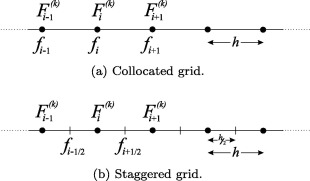
\includegraphics[width=0.7\linewidth]{img/spectral_theory/staggered_grid.jpg}
\end{figure}

\begin{enumerate}
	\item Discretize the equation on the OPPOSITE grid where the function $v$ is defined on.
	\item Discretize the equation on the SAME grid where the function $v$ is defined on.
\end{enumerate}


If we assume $v\sim \exp(-ikx)$, and let $\beta\equiv kh/2$. Then the differential operators $\dv*[n]{x}$ are equivalent to the following factors \cite{llobet_spectral_1990},
\begin{itemize}
	\item Evaluate equation on the OPPOSITE grid
	align
	\begin{align}
		&H_0 = [\exp(i\beta)+\exp(-i\beta)]/2 = \cos(2\beta) \nonumber \\
		&H_1 = [\exp(i\beta)-\exp(-i\beta)]/h = (2i/h)\sin(\beta) 
		\label{H-operator} \\
		&H_2 = [\exp(3i\beta)-\exp(i\beta)-\exp(i\beta)+\exp(-3i\beta)]/2h^2 = H_1^2H_0 \nonumber 
	\end{align}
	
	\item Evaluate equation on the SAME grid
	\begin{align}
		&G_0 = 1 \nonumber \\
		&G_1 = [\exp(2i\beta)-\exp(-2i\beta)]/2h = (i/h)\sin(2\beta) = H_1H_0 
		\label{G-operator}\\
		&G_2 = [\exp(2i\beta)-2-\exp(-2i\beta)]/h^2 = (2/h^2)(\cos(2\beta)-1) = H_1^2 \nonumber 
	\end{align}
\end{itemize}


\subsection{Analysis of Numerical Spectrum}
\subsubsection{Discretize on the Same Grid}
Using the G-operator, Eq.(\ref{G-operator}), the discretized equation of Eq.(\ref{polynomial-eigenvalue-problem}) is 
\[ \omega^2 + \omega(2iv_0H_1H_0) + (1-v_0^2)H_1^2 = 0 \]

Thus the numerical dispersion relation is
\begin{equation} \label{dispersion-relation-G}
	\omega = -iH_1 \left(v_0 \pm \sqrt{v_0^2H_0^2 + (1-v_0^2)}\right) = \frac{2\sin(\beta)}{h}\left(v_0 \pm \sqrt{1 - v_0^2\sin[2](\beta)}\right)
\end{equation}

We see that 
\begin{itemize}
	\item $\omega$ is real for all $k$ if $v_0 < 1$.
	\item $\omega$ is complex for large $k$, more specifically $k>h/2\arcsin(1/v_0)$, if $v_0 > 1$.
	\item For small $k$, meaning $k\to 0$, Eq.(\ref{dispersion-relation-G}) is a good representation for the analytical dispersion relation, Eq.(\ref{dispersion-relation}). 
\end{itemize}
This explains why the spurious unstable modes occur when $v_0>1$.


\begin{figure}[H]
	\centering
	\begin{subfigure}[b]{0.5\linewidth}
		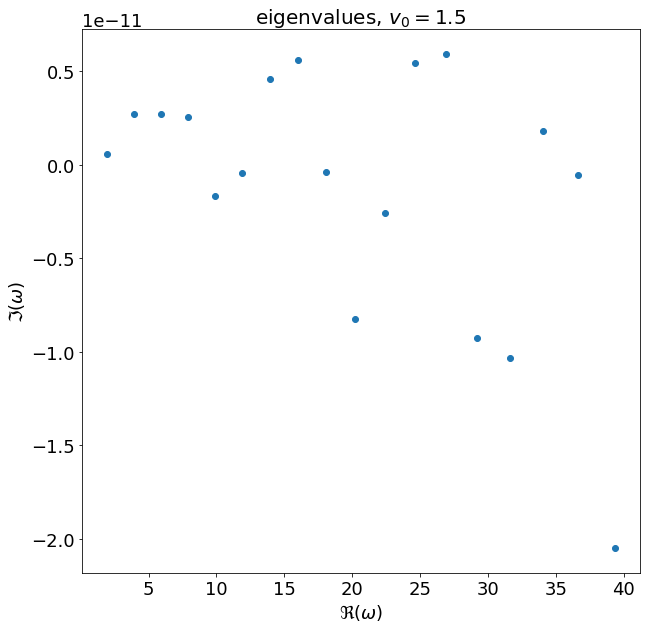
\includegraphics[width=\linewidth]{img/spectral_theory/eigvals_G_filtered.png} 
		\caption{Filtered eigenvalues}
		\label{fig:results-G-a}
	\end{subfigure}%
	\begin{subfigure}[b]{0.5\linewidth}
		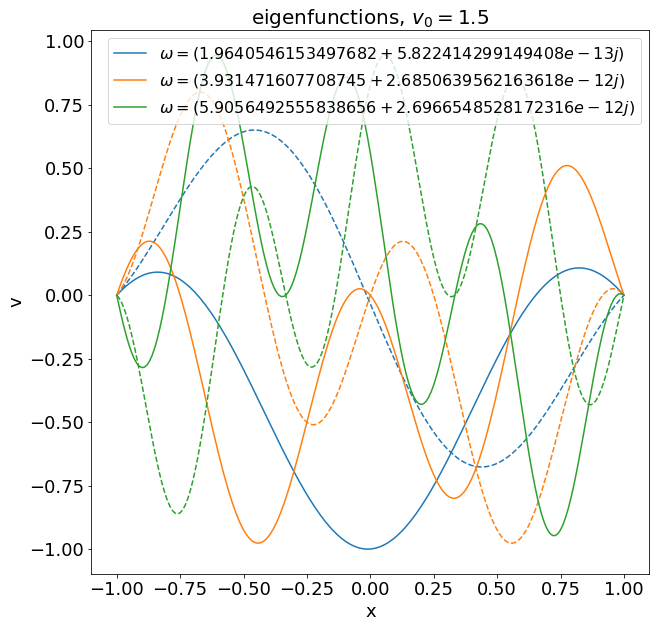
\includegraphics[width=\linewidth]{img/spectral_theory/eigfuncs_G_filtered.png} 
		\caption{Filtered eigenfunctions}
		\label{fig:results-G-b}
	\end{subfigure}
	\caption{Filter out the spurious modes with $k>h/2\arcsin(1/v_0)$.}
	\label{fig:results-G}
\end{figure}

\subsubsection{Discretize on the Opposite Grid}
Using the H-operator, Eq.(\ref{H-operator}), Eq.(\ref{polynomial-eigenvalue-problem}) becomes
\[ \omega^2H_0 + \omega(2iv_0H_1) + (1-v_0^2)H_1^2H_0 = 0 \]

So the numerical dispersion relation is
\begin{equation}\label{dispersion-relation-H}
	\omega = -iH_1 \left(v_0 \pm \sqrt{v_0^2 + (1-v_0^2)H_0^2}\right) = \frac{2\sin(\beta)}{h}\left(v_0 \pm \sqrt{\cos[2](\beta) + v_0^2\sin[2](\beta)}\right)
\end{equation}

We see that 
\begin{itemize}
	\item $\omega$ is real for all $k$ for all $v_0$.
	\item For small $k$, Eq.(\ref{dispersion-relation-H}) dramatically deviates from the analytical dispersion relation Eq.(\ref{dispersion-relation}). 
\end{itemize}

\begin{figure}[H]
	\centering
	\begin{subfigure}[b]{0.3\linewidth}
		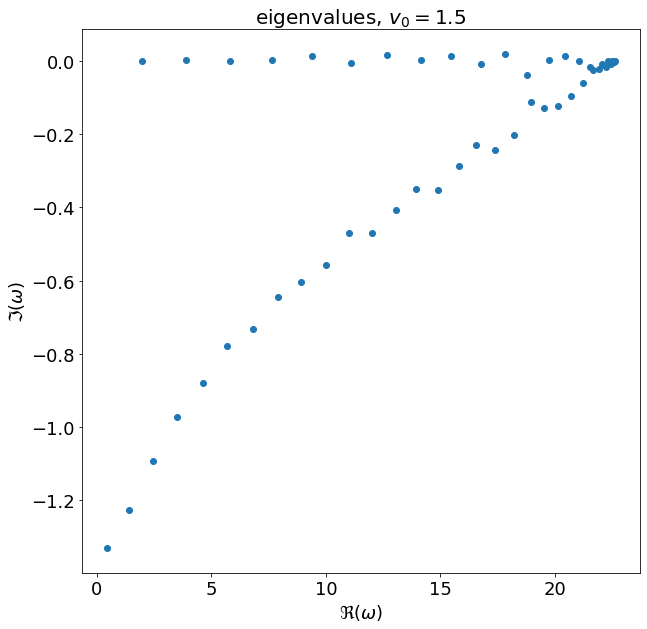
\includegraphics[width=\linewidth]{img/spectral_theory/eigvals_H.png} 
		\caption{Deformed eigenvalues, accumulation point occurs.}
		\label{fig:results-H-a}
	\end{subfigure}
	\begin{subfigure}[b]{0.3\linewidth}
		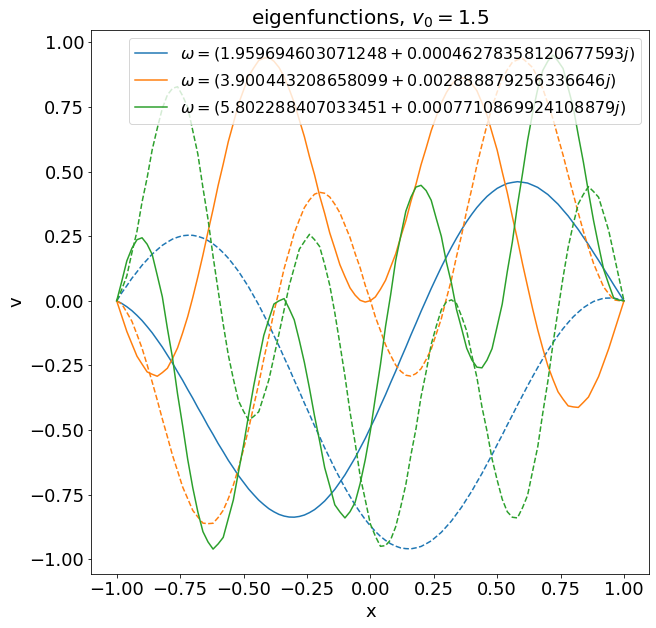
\includegraphics[width=\linewidth]{img/spectral_theory/eigfuncs_good_H.png} 
		\caption{Good eigenfunctions}
		\label{fig:results-H-b}
	\end{subfigure}
	\begin{subfigure}[b]{0.3\linewidth}
		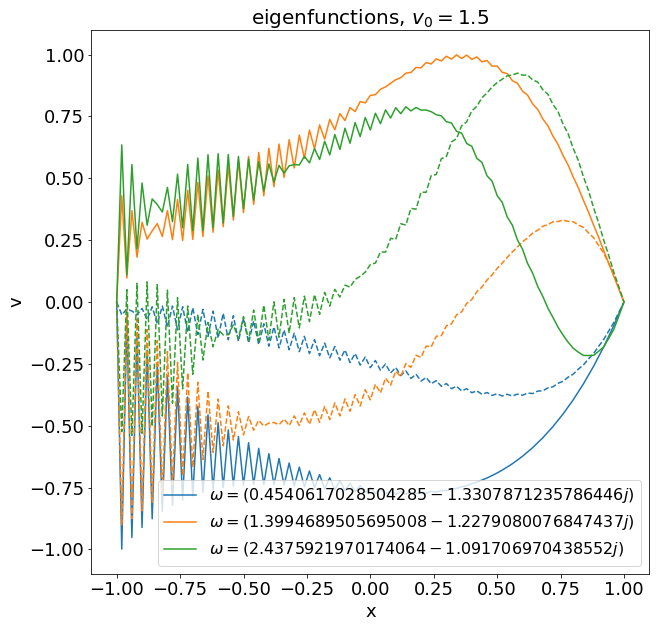
\includegraphics[width=\linewidth]{img/spectral_theory/eigfuncs_bad_H.png}
		\caption{Spurious modes.} 
		\label{fig:results-H-c}  
	\end{subfigure}
	\caption{Although the spurious unstable modes are much smaller, but the eigenvalues deviate from the analytical dispersion relation.}
	\label{fig:results-H}
\end{figure}

\subsection{Conclusion}
\begin{enumerate}
	\item If we discretize Eq.(\ref{polynomial-eigenvalue-problem}) on the same grid as the function $v$ is defined on, then the eigenvalues are good for small $k$ modes. To get the good modes, we can filter out the modes with wave number $k>h/2\arcsin(1/v_0)$.
	\item While we get less spurious unstable modes if we discretize Eq.(\ref{polynomial-eigenvalue-problem}) on the opposite grid as the $v$ is defined on, we suffer the inaccurate eigenvalues.
\end{enumerate}